
\begin{textarea}[]
  \only<1>{
    \begin{algorithm}[H]
      \begin{algorithmic}[1]
        \FOR {$k = 1 \cdots n$}
        \FOR {$i = k+1 \cdots n$}
        \STATE $m := A[i, k] / A[k, k]$
        \FOR {$j = k+1 \cdots n$}
        \STATE $A[i, j]  := A[i, j] - A[k, j] * m$
      \ENDFOR
      \STATE $A[i, k]  := 0$
    \ENDFOR
  \ENDFOR
\end{algorithmic}
\end{algorithm}
}
\only<2>{
  What is the Gauss-Algorithm?
}
\end{textarea}




\begin{textarea}[]
	\only<1>{
		\begin{algorithm}[H]
			\textbf{FUNCTION} F(n)
			\begin{algorithmic}[1]
				\IF{$n \leq 1$}
				\RETURN $n$
				\ELSE
				\RETURN $F(n-1)+F(n-2)$
				\ENDIF
			\end{algorithmic}
		\end{algorithm}
	}
	\only<2>{
		What is the Fibonacci Algorithm?
	}
\end{textarea}




\begin{textarea}[]
	\only<1>{	
		%\includemovie{5cm}{5cm}{media/code/code/Merge-sort-example-300px.gif}
		\animategraphics{80}{categories/media/code/Merge-}{0}{211}
	}
	\only<2>{
		What is Mergesort.
	}
\end{textarea}


\begin{textarea}[]
	\only<1>{
		\centering
		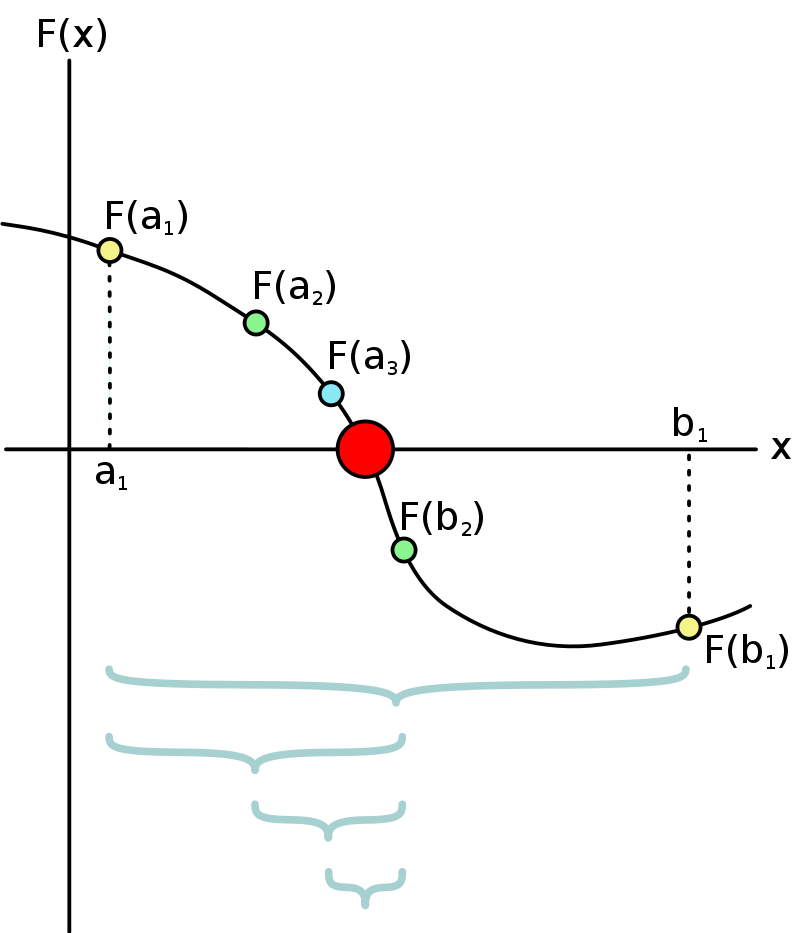
\includegraphics[height=0.5\linewidth]{categories/media/code/800px-Bisection_method}
	}
	\only<2>{
		What is the Bisection Algorithm?
	}
\end{textarea}


